\documentclass[twoside]{article}


% ------
% Fonts and typesetting settings
\usepackage[sc]{mathpazo}
\usepackage[T1]{fontenc}
\linespread{1.05} % Palatino needs more space between lines
\usepackage{microtype}
\usepackage{verbatim}
\usepackage[utf8]{inputenc} % Enable Umlaute
\usepackage{amsmath}
\usepackage{graphicx}

% ------
% Page layout
\usepackage[hmarginratio=1:1,top=32mm,columnsep=20pt]{geometry}
\usepackage[font=it]{caption}
\usepackage{paralist}
\usepackage{multicol}
\usepackage{natbib}

% ------
% Lettrines
\usepackage{lettrine}


% ------
% Abstract
\usepackage{abstract}
	\renewcommand{\abstractnamefont}{\normalfont\bfseries}
	\renewcommand{\abstracttextfont}{\normalfont\small\itshape}


% ------
% Titling (section/subsection)
%\usepackage{titlesec}
%\renewcommand\thesection{\Roman{section}}
%\titleformat{\section}[block]{\large\scshape\centering}{\thesection.}{1em}{}


% ------
% Header/footer
\usepackage{fancyhdr}
	\pagestyle{fancy}
	\fancyhead{}
	\fancyfoot{}
	\fancyhead[C]{Trends in Artificial Intelligence $\bullet$ Research Proposal $\bullet$ \today }
	\fancyfoot[RO,LE]{\thepage}


% ------
% Clickable URLs (optional)
\usepackage{hyperref}


% ------
% Maketitle metadata
\title{\vspace{-15mm}%
	\fontsize{24pt}{10pt}\selectfont
	\textbf{Sales conversation analysis using topic modelling in conjunction with empathy detection}\\
	}	
\author{%
		 \begin{tabular}{rl}
  Student name:& Christoph Schmidl\\ 
  Student number:& 4226887 \\ 
  E-mail address:& \href{mailto:c.schmidl@student.ru.nl}{c.schmidl@student.ru.nl}\\
  Theme:& Cognitive models for understanding  \\ &language and web data\\
 \end{tabular}\\
	%\vspace{-5mm}
	}
\date{}



%%%%%%%%%%%%%%%%%%%%%%%%
\begin{document}

\maketitle
\thispagestyle{fancy}

  \begin{center}
  	Radboud University, Nijmegen  
  \end{center}  
  \vspace{2.5mm}

\begin{abstract}

\noindent Sales conversations between a so-called seller and a potential customer over the phone can result into a successful and a failed conversion in the very end. Empathy and Topic Divergence between a seller and a potentical customer seem to be important features which correlate with a successful conversion. This research tries to confirm this belief by using Natural Language Processing Techniques on raw audio but also on textual data by using the openSMILE library and its empathy detection module and Latent Dirichlet Allocation for topic divergence discovery.
\end{abstract}



\begin{multicols}{2}



\section{Project Description}

\subsection{Background}

Companies like Deutsche Telekom record each conversation between their salesforce and possibly clients over the phone. It can be assumed that  companies which rely heavily on their salesforce team leveraging client contact by phone also label these conversations with regards to a successful or failed sale. According to \cite{effectiveSalesConversations2018}, there are certain guidelines for sellers which make phone calls more probable in leading to a successful sell at the very end. One of these guidelines suggests maintaining a certain level of empathy but also staying on topic with regards to the domain of the companie's products. Extracting verbal and phonetic features could be indicators for a successful sell. Manual analysis of these conversations would not be cost effective and furthermore cumbersome.\\
Natural Language Processing (NLP) has come a long way since the introduction of techniques like part-of-speech tagging (POS tagging), chunking, named entity recognition, and semantic role labeling as it is proposed in \cite{Collobert2011}. More sophisticated NLP techniques could help to extract those features which lead to a successful sale.


\subsection{Sales Conversations}

Conversations between two humans over the phone is a common thing. Sales conversations on the other hand are special in the case that one party represents a seller and the other party a potential customer. A sales conversation phone call can have two different results: successful or failed sell of a service or product. Sales conversations are usually recorded in one file where the parties are not split into separate channels. The different parties, also called speakers are also often speaking at the same time and are interrupting each other or overlapping. This represents another problem when transcripting audio files into textual representations to make NLP techniques applicable. 


\subsection{Natural Language Processing}

NLP is usually applied to textual data and not to audio data. To apply NLP techniques to the before mentioned audio files / sales conversations, the conversations have to be transribed from audio to text. The openSMILE library is an open source tool which seems to be fitting for this kind of problem and has been used by \cite{Eyben2013} before. This library provides functionality like an automatic speech recognition module (ASR) and is therefore able to perform speaker diarization and transcribing audio to text. From this point on it would be possible to apply different NLP techniques but also use functionality from the openSMILE library to analyse phonetic features on raw audio.\\
\cite{Alam2017} used the openSMILE library for modelling levels of empathy in human-to-human dyadic spoken conversations. Like stated before, the success rate of a sales conversation seems to be highly influenced by the level of empathy between seller and customer and can be used for this research. Their proposed pipeline seems promising and applicable to this research, see Figure \ref{classification-pipeline}.

\begin{center}
  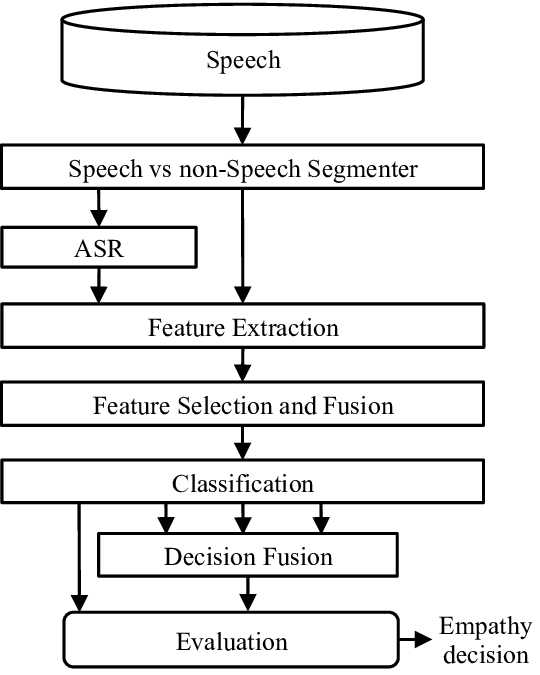
\includegraphics[height=70mm]{images/pipeline.png}
  \captionof{figure}{The empathy classification system}
  \label{classification-pipeline}
\end{center}



Another feature which seems to be important for successful sales conversations is the divergence between topics which have been mentioned by the seller and the customer. There are different probabilistic topic models available like proposed in \cite{topicmodels2007} where Latent Dirichlet Allocation seems to be the most common one.


\subsection{Research Question}

Based on a rule of thumb proposed by different sources while one was mentioned in the beginning \cite{effectiveSalesConversations2018}, Empathy and topic matching between two speakers seem to be important features for a successful sales conversation. There has been no prior research which confirms these statements using NLP techniques. Therefore there are two research questions which emerge from this:

\begin{itemize}
	\item Is the level of empathy between a seller and potential customer an important feature which leads to a higher rate in successful sales conversations?
	\item Is topic divergence between a seller and potentical customer an important feature which leeads to a higher rate in successful sales conversations?
\end{itemize}

In order to answer these questions, this research will use techniques from \cite{Alam2017} for detecting empathy and \cite{topicmodels2007} to calculate topic divergence.



\subsection{Research Plan}

To answer the before mentioned questions the research will go through different phases. The first phase will concentrate on gathering suitable data in the form of audio files of sales conversation phone calls. To my knowledge there is no freely available dataset of sales conversations. However, \cite{Lowe2015} is providing a large dataset for research in unstructured multi-turn dialoque system and \cite{Moviedic} offers a movie dialogue corpus for research and development. These two could be used as a fallback plan if there is no company available which would be interested in a proof-of-concept collaboration to this research. I assume that there will be an interested company withing the timeframe of one month which would be willing to share an anonymized subset of their sales conversations. Having labels which indicate a successful and failed conversation is crucial for this research.


\subsubsection{The experiment}

After collecting the dataset in the form of audio files where each audio file contains two speakers, namely seller and customer, with labels indicating a successful or failed sales conversation, the second phase starts.\\
The second phase will concentrate on annotating the dataset. Annotation will be performed on the whole dataset using Amazon Mechanical Turk with regards to empathy like it is proposed in \cite{Alam2017} and the number of perceived topics for later evaluation of the correct value of $k$ topics in LDA. Empathy in this context is defined by the definition of \cite{Hoffman2008}, where "an emotional state triggered by another's emotional state or situation, in which one feels what the other feels or would normally be expected to feel in his situation".\\
The third phase will split the dataset into 70\% training, 20\% validation  and 10\% test set where a cross-validation approach will be used later on, so that every sample gets a chance to be contained in one of the sets at least once.
The fourth phase will use the openSMILE library to generate empathy profiles of a sample between a seller and a potential customer. Empathy detection will be implemented by using the pipleline of openSMILE as seen in Figure \ref{classification-pipeline}. Furthermore, Latent Dirichlet Allocation will be used to identify the topics generated by the seller and by the customer. The main problem here is the fact that LDA requires prior knowledge in terms of the number of topics to cluster. Because we do not have this knowledge, different values for $k$ will be used and then the one will be selected that has the largest likelihood. Another approach would be to use Hierarchical Dirichlet Process (HDP) instead of LDA because it does not require a fixed value for the number of topics but we will stick to LDA based on the fact that it is the most common topic modelling technique and it makes the results comparable to other approaches.\\
The fifth phase will compare the manually annoated labels by Amazon Mechanical Turk regarding empathy levels and topics against the automatic approach using the openSMILE library and LDA. The results of both approaches will then be compared based on their agreement level using Cohen's kappa. Samples with a high agreement level will then be selected as input features for a classifiers like a Support Vector Machine with a linear kernel to estimate feature importance with regards to successful sales conversation or failed sales conversation. A linear kernel is required to apply techniques like recursive feature elimination in order to plot feature importance.



\subsubsection{Data Analysis}

The analysis of the data will be performed in different steps. One step involves the analysis of manually annotated data based on the number of topics $k$ and the empathy annotations based on the modal model of emotions from \cite{Alam2017}.\\
The other step involves the anaysis of the automatic approach using LDA and the openSMILE library. In this step the value for $k$ for LDA will be chosen based on the largest likelihood and the openSMILE library will give empathy levels using the proposed pipeline.\\
We then have two different annoations and different values for $k$ for each sample and can calculate the agreement between these two using Cohen's Kappa.

\begin{align}
\kappa = \frac{p_0 - p_e}{1 - p_e} = 1 - \frac{1 - p_o}{1 - p_e}
\end{align}

Cohen's Kappa shows in how far two annotators agree taking into account that the agreement could occur by chance. A certain threshold is used to determine the optimal value for $k$ and empathy agreements. The resulting subset of data with a high agreement level can then be used for further analysis.\\

After choosing a value for $k$, the resulting topic distributions between the seller and the customer in each sample can be calculated and later on compared using Kullback Leibler (divergence) or Jensen-Shannon (JS) divergence.\\

Accoring to \cite{topicmodels2007}, \textit{the Kullback Leibler (KL) divergence is a standard function to measure the difference between two distributions} $p$ and $q$.

\begin{equation}
	D(p,q) = \sum_{j=1}^T p_j \log_2 \frac{p_j}{q_j}
\end{equation}

\textit{This non-negative function is equal to zero when for all} $j, p_j = q_j$. \textit{The KL divergence is asymmetric and in many applications, it is convenient to apply a symmetric measure based on KL divergence.}

\begin{align}
	KL(p,q) = \frac{1}{2} [ D(p,q) + D(p,q)]
\end{align}

\textit{Another option is to apply the symmetrized Jensen-Shannon (JS) divergence:}

\begin{align*}
	JS(p,q) &= 
\end{align*}
\vspace{-20 pt}
\begin{align}
	 \frac{1}{2} [D(p,(p + q)/2) + D(q, (p + q)/2)]
\end{align}


The modal model of emotions can serve as a general framework to compare empathy levels to each other \cite{Alam2017}.\\

After performing these steps, the resulting scores for empathy levels and distribution convergence can serve as input features for a Support Vector Machine with a linear kernel which serves as a binary classifier for successful and failed sale conversations. This step is necessary to see if empathy and topic divergence are indeed important features which correlate with successful sales conversations.


\section{Schedule}

The project is intended as a Master thesis and therefore contains a timeframe of six months which are approximated 24 weeks. Six weeks are added as a buffer.

\begin{center}
\begin{tabular}{ |c|c| } 
 \hline
Collecting dataset & Deadline: week 4 \\ 
Annotating dataset & Deadline: week 6 \\ 
Implementing pipeline & Deadline: week 12 \\
Data Analysis & Deadline: week 22 \\
Write thesis & Deadline: week 30 \\ 
 \hline
\end{tabular}
\end{center}
 


\section{Relevance}

Sales conversation analysis is a growing market based on the fact that NLP techniques are getting more sophisticated and computing power gets cheaper. More powerful GPUs and the rise of deep learning techniques also make this business model more attractive because most of the time they are more precise and also cheaper than manual, human analysis. Although this research does not seem to have a major scientific impact it seems to offer potential for a business model which concentrates on conversation analysis based on empathy and topic modelling as their main features which could correlate with conversion rate. Other features could be added later on easily and evaluated for their contribution to a successful sales conversation. These insights later on could be used to train a salesforce team to maximize their profits by improving their skills based on analysis methods proposed during this research.



\bibliography{myrefs}{}
\bibliographystyle{apa}





\end{multicols}

\end{document}
